\documentclass[10pt,a4paper, twocolumn]{report}
\usepackage[utf8]{inputenc} 
\usepackage[spanish]{babel}
\usepackage{amsmath}
\usepackage{amsfonts}
\usepackage{amssymb}
\usepackage{graphicx}
\usepackage{multirow}
\author{Antonio Molina García-Retamero}
\title{Optimización de redes neuronales mediante métodos bioinspirados}
\makeindex
\begin{document}
\onecolumn
\maketitle
\pagebreak
\tableofcontents
\pagebreak

\chapter{Introduction}
\section{La propuesta de Trabajo de Fin de Grado}
En este documento se recoge la memoria del trabajo de fin de grado que he realizado y que pretende justificar los valores y facultades adquiridas en el estudio y superación de las competencias recogidas en el Grado en Ingeniería Informática. En estas primeras líneas trataré de exponer el trabajo en términos generales y justificar la elección del mismo y las bondades y problemas del mismo.

\subsection{Justificación y objetivos}
En el proceso de elección del proyecto de fin de grado y de los objetivos a plantear para el desarrollo del mismo, he de indicar que primó mi clara vocación investigadora y es por ello que desde el principio le planteé a mi tutor del proyecto mi deseo de realizar algún tipo de investigación básica, con especial interés es el campo de la inteligencia artificial. Es por eso que este proyecto de fin de grado está generalmente enfocado al desarrollo de una investigación que pueda encontrar una aplicación práctica evidente y que cubra en la medida de lo posible todas las competencias adquiridas durante el grado. Por lo tanto, los objetivos generales que cubren este trabajo serían:
\begin{itemize}
	\item Búsqueda de un problema relativo al campo de estudio sobre el que realizar un proceso investigador con tal de dar solución al problema desde un punto cientifico-técnico.
	\item Estudio del estado del arte del problema en cuestión.
	\item Planteamiento de soluciones.
	\item Experimentación.
\end{itemize}

\fbox{Aquí no sé si debería decir que el objetivo último es la elaboración de un artículo}

La redacción de esta memoria está estructurada haciendo una división entre el trabajo puramente teórico e investigador que será la primera parte de la misma y que tratará de clarificar la metodología de investigación, el planteamiento del problema objeto de estudio y el estudio del estado del arte. En la segunda parte se tratará el diseño y la implementación del banco de pruebas sobre el que realizar el proceso experimentador y se justificará la elección de las tecnologías y metodologías utilizadas. En la tercera parte de esta memoria se detallará la experimentación realizada, se recogerán los resultados y se detallarán las conclusiones del trabajo en su conjunto. 

\section{Proceso de investigacion}
\subsection{Planteamiento del problema}
Una vez definido el trabajo y planteados los objetivos del mismo, el siguiente paso ha sido determinar el problema que se va a tratar dentro del proceso investigador y así tratar de proponer una solución al problema siguiendo una metodología de investigación.
Las redes neuronales, por su propia naturaleza, han pretendido de alguna manera emular el proceso cognitivo que se produce en el cerebro de los mamimeros, siempre a una escala reducida, pero sirviéndose de los mismos principios fundamentales. Sin embargo, el problema del aprendizaje es tradicionalmente objeto de la estadísticas y no de la biología. Las redes neuronales aplicadas a problemas de aprendizaje han sido muy estudiadas como un problema estadístico y existe una muy extensa literatura al respecto, sin embargo, no ha sido hasta años recientes que se está abordando el problema del aprendizaje máquina desde un punto de vista biológico. En los últimos años, la neurocomputación ha adquirido una muy notable importancia dentro del campo del aprendizaje máquina y propone sistemas que realmente pretenden emular a los sistemas biológicos y en los que la posibilidad de llegar a entender quizá un poco más los procesos que dotan a los sistemas biológicos de inteligencia y quizá incluso emular algunas de sus funcionalidades es un campo muy prometedor y cargado de retos ilusionantes.

Partiendo del problema de tratar de emular mecanismos biológicos en los modelos de aprendizaje máquina, mi tutor, Daniel Ruiz, me mostró el trabajo de Diego Andina sobre la aplicación de la metaplasticidad neuronal al perceptrón multicapa (MLP) y me propuso el aplicarlo a otro tipo de redes como las RBFNN.

\subsection{El estado del arte}
Dado que partimos de un trabajo en curso, que es la implementación de la metaplasticidad artificial en redes neuronales artificiales, el estudio del estado del arte ha sido un trabajo áurduo que ha requerido de un estudio bastante en profundidad de las diferentes disciplinas bajo las que se contempla el problema que hemos definido y que cubren desde la neurobiología a la estadística y el aprendizaje máquina. Es por esto que me serviré de esta sección primero para demostrar de alguna forma el trabajo realizado en la documentación y adquisición de conocimientos necesarios para comprender el problema y plantear una solución así como para tratar de introducir al lector, de la forma más amena posible, en los conceptos y terminología en que se definen la problemática y la solución propuesta al problema.

El trabajo se inicia con el estudio de lo relativo a la metaplasticidad en las redes neuronales biológicas. Además, he dedicado tiempo a estudiar y entender los modelos estadísticos bajo los que se estudian las redes neuronales artificiales para buscar la forma de aplicar este principio, que es la metaplasticidad artificial, a otros tipos de redes neuronales artificiales más allá, y partiendo, del trabajo que ha desarrollado Diego Andina en las MLP.

En las siguientes subsecciones se definirán primero la metaplasticidad en términos biológicos para después explicar

Una vez adquiridos los conocimientos necesarios para comprender el problema, se realizará un estudio del estado del arte de las diferentes técnicas de las RBFNN con tal de encontrar la forma de aplicar el concepto de metaplasticidad que se da de forma natural en las redes neuronales biológicas.

En este punto de la investigación se ha recurrido de nuevo a la bioinspiración tratando de encontrar una perspectiva bajo la que contemplar las RBFNN y sobre la que plantear una solución al problema. 

\fbox{
	Aquí quiero decir que el tema de RBFN como "kernel methods" y lo de la tonotopy y retinotopy, que es también estado del arte, lo trato más adelante como una ampliación del estado del arte, para no meter más conceptos aquí y que tiene más coherencia explicarlo cuando propongo la solución.
}

\subsection{La metaplasticidad en redes biológicas}
Metaplasticity refers to activity-dependent changes in neural functions that modulate subsequent synaptic plasticity such as long-term potentiation (LTP) and long-term depression (LTD). Simply put, it is the “plasticity of synaptic plasticity” (Abraham and Bear, 1996). Metaplasticity can be distinguished from conventional neuromodulation of plasticity, in which molecules such as other neurotransmitters (e.g., GABA or monoamines), cytokines, or hormones that are present at the time of plasticity induction regulate the degree of LTP or LTD elicited (Fig. 1). Metaplasticity, in contrast, refers to neuronal changes that are elicited at one point in time, by what is commonly called “priming” activity. By virtue of their persistence, these neuronal changes are able to regulate synaptic plasticity processes minutes, hours, or days later. At very short intervals between priming activity and plasticity induction, however, the distinction between metaplasticity and neuromodulation may become blurred. In many cases, metaplasticity is induced without producing observable changes in synaptic transmission, and it only becomes apparent during subsequent attempts to induce LTP or LTD. In practice, however, neural activity can generate metaplasticity concomitantly with synaptic plasticity.

Functionally, metaplasticity endows synapses with the capacity to integrate plasticity-relevant signals across time. It can also serve, by changing the thresholds for LTP and LTD, to keep synaptic strengths within a functional dynamic range. That is, it prevents them from becoming so strong or weak that they lead to excessive or insufficient activation, respectively, of the postsynaptic cells. Readers are directed to a recent review for a more comprehensive discussion of metaplasticity (Abraham, 2008). 

Con el término metaplasticidad nos referimos al cambio dependiente de la actividad que modula la plasticidad sináptica en los sistemas neuronales. Estos cambios en la plasticidad pueden ser del tipo LTP (long-term potentiation) y LTD (long-term depression).
\section{Metaplasticidad en redes neuronales artificiales}
\chapter{Metaplasticidad en Redes Neuronales con Función de Base Radial (RBFNN)}
\subsection{Propuesta de solución}
\section{Mi intuición de metaplasticidad en RBFNN}
En base a los trabajos previos, la idea de servirnos de la naturaleza de los datos de nuestro entrenamiento para hacernos una idea a priori de cuan significativa es una muestra y actuar ponderando esa "conexión sináptica" concreta parece encajar de forma especial en el concepto de RBFNN debido a la naturaleza de las Funciones de Base Radial. Quiero decir, las Funciones de Base Radial nos proporcionan una transformación no lineal que nos permite encontrar un hiperplano que en algún espacio multidimensional nuestros datos serán separables. El modelo de las RBFNN, como ya hemos comentado, se sirven de un modelo con la forma $f(x)=\sum w \phi(x)$ donde $\phi(x)$ es un función de base radial. Este tipo de funciones pueden ser muy variadas y se ha experimentado con multitud de ideas alrededor de esto sin embargo en los casos más habituales se utiliza una función gausiana en donde tenemos que inferir tanto la media como los centroides para cada una de las funciones en nuestro training set. De esto se deriva un entrenamiento de dos fases en el que en la primera fase inferimos los datos necesarios para calcular la activación de la capa oculta para hacer luego encontrar los parámetros para la transformación lineal sobre la salida de esta capa en una segunda fase de entrenamiento.

Aquí es donde pretendo encontrar y probar diferentes formas de optimizar la segunda fase de entrenamiento sirviéndonos del estudio estádico que implica la primera fase. Esto es, Cuando en la primera fase de entrenamiento buscamos los centros para nuestras funciones de activación obtenemos información relevante que podemos utilizar para estimar, como hablábamos antes, como considerar una probabilidad de pertenencia a una clase si consideramos el centroide como una clase, etc... Multitud de ideas se pueden considerar y en última instancia lo que se estaría haciendo sería entremezclar de diferentes formas el proceso de aprendizaje no supervisado a priori para influir en el proceso de aprendizaje supervisado de la segunda fase.


\chapter{Implementación}
Tendría que encontrar el sitio donde poner qué se ha implementado y por qué
\section{Metodología de desarrollo}
Aquí comento que he realizado la implementación siguiendo el paradigma TDD para la implementación de las redes.
\section{Lenguaje y herramientas}
\section{Implementación de las redes}
\section{Pruebas y métricas de rendimiento}
Dado que por medio de este trabajo se pretende la demostración de la mejora propuesta sobre las RBFNN, estableceré una serie de pruebas que pretenderán poner a prueba las diferentes implementaciones de las redes para resolver problemas típicos de aprendizaje máquina.
En secciones anteriores hemos comentado la problemática y las diferentes alternativas propuestas para entrenar las RBFNN. La batería de pruebas es la parte probablemente más crítica del proyecto y con especial esmero he diseñado un conjunto de pruebas que pretende ser exhaustivo y con el que pretendo primero valorar el comportamiento de las soluciones típicas existentes y las mejoras propuestas en esta investigación.

De entre los escenarios típicos del aprendizaje máquina podemos hacer dos grandes grupos: tal y clasificación. Para este proyecto he seguido la estrategia de construir, para sendos tipos de problemas, sets de datos aleatorios cuyos parámetros intrínsecos puedan ser manipulados fácilmente permitiendo generar de forma sencilla tantos escenarios como se crean apropiados para los diferentes test. En busca de evitar el "data snooping" y una vez determinadas las configuraciones para los que los diferentes tipos de redes tienen comportamientos interesantes, las redes serán testeados sobre sets de datos estándares en la investigación sobre aprendizaje máquina.

\begin{itemize}
	\item Reconocimiento de patrones
	\begin{itemize}
		\item Onda compuesta aleatoria
		\item Otra idea que se me ocurra
	\end{itemize}
	\item Clasificación
	\begin{itemize}
		\item Clasificación sobre datos aleatorios artificiales
		\item Clasificación sobre datos reales
	\end{itemize}
\end{itemize} 
En las siguientes secciones trataré de clarificar todo esto para cada tipo de pruebas. Explicaré las cosas fundamentales de la implementación tratando de no perder al lector en el código pero dándo una visión clara y precisa de lo que se desea poner a prueba con cada test. Sin embargo, antes de entrar en detalle sobre la construcción de los conjuntos de datos me gustaría dejar patente el guión básico que sigo a la hora de diseñar las prubas.

Anteriormente hemos discutido las fases del entrenamiento de redes RBFNN y de las soluciones típicas. Además discutimos acerca de como podemos implementar la intuición de la metaplasticidad en la fase supervisada a partir de la información estadística que supone el aprendizaje no supervisado de la primera parte del entrenamiento en busca de los parámetros de las funciones de base radial. 

Con todo esto, una primera batería de test tratará de determinar en qué condiciones, el cálculo de la pseudoinversa deja de resultar rentable en términos de coste computacional con respecto a al descenso por gradiente. Este coste computacional es directamente proporcional al tamaño del set de datos, con lo que esta prueba nos dará una estimación de cuan grande ha de ser al menos nuestro conjunto de datos para que resulte rentable la aproximación del descenso por gradiente que es necesario para la implementación de la intuición de metaplasticidad aquí propuesta.

A continuación, someteremos a una batería exahustiva de test generados artificialmente y sobre los que variaré los parámetros de los diferentes tipos de redes y de los propios conjuntos de datos en busca de las condiciones en que cada tipo de RBFNNs de los propuestos ofrece un comportamiento mejor que el resto. Con esto podremos determinar si existen condiciones en las que, en efecto, la propuesta de metaplasticidad supone una mejora sobre las aproximaciones existentes.

Por último, se realizarán pruebas sobre sets de datos conocidos y ampliamente utilizados en el campo del aprendizaje máquina. Con esto se pretende evitar la aparición de resultados inválidos por la propia intervención y manipulación de los parámetros y datos en busca de las condiciones en las que la esta implementación resulte mejor además de poder ofrecer comparativas que puedan ser reconocidas por quienes trabajan en otras propuestas sobre los mismos conjuntos de datos.

\subsection{Pruebas de clasificación}
Uno de los usos más habituales de las RBFNN es cuando tenemos que clasificar sobre un conjunto de datos cuyas clases no son linealmente separables. Anteriormente hablamos de
\begin{figure}[!h]{}
    \centering
    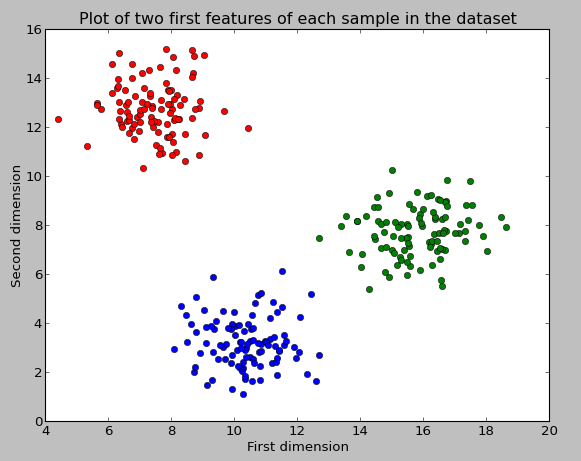
\includegraphics[width=0.4\textwidth]{img/clusteredData1.png}
    \label{fig:clusteredData1}
    \caption{Conjunto de datos con distribución normal}
\end{figure}
Ya que, a través de las RBFNN, obtenemos un modelo con la forma $f(x)=\sum w_{i}\phi(r)$ (que es caracterizado con funciones de base radial) podemos aproximar funciones complejas cuya salida sigue una distribución gaussiana (la más frecuente con mucha diferencia de entre las variables aleatorias que se dan en la naturaleza) con notable precisión. 
La figura \ref{fig:clusteredData1} es un ejemplo de datos generados con el generador de datos clusterizados que he implementado. Este recibe como parámetros básicos el número de centroides y el número de muestras y genera estos datos de forma aleatoria tomando como centro los k-centroides también tomados aleatoriamente. En las siguientes líneas introduciré esta clase sin entrar en excesivo detalle de la implementación pero sí tratando de aclarar las cuestiones que considero claves.

\subsubsection{Generación de datos aleatorios}
Para este tipo de test necesitamos generar datos que se distribuyan de forma normal alrededor de un centroide. Una distribución normal es aquella que cuya función de densidad de probabilidad queda definida por la media ($\mu$) y la desviación estándar ($\sigma$) del conjunto de datos ($x$) de la siguiente forma:
\begin{center}
$pdf(x,\mu,\sigma) = \frac{1}{ \sigma \sqrt{2 \pi}} e^{\left(-\frac{{\left(\mu - x\right)}^{2}}{2 \, \sigma^{2}}\right)}$
\end{center} 
Existen multitud de generadores aleatorios de este tipo de datos. En este caso utilizaré el propio de NumPy como muestro a continuación para generar las $n$ muestras por cada centroide ya que este definirá la media. La desviación estándard será proporcionada como parámetro en el constructor de la clase y nos permitirá jugar con la forma que adoptarán los datos generados.

\begin{figure}[!h]{}
    \centering
    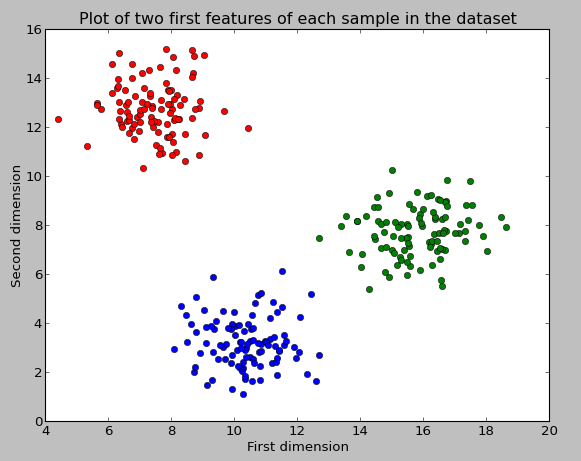
\includegraphics[width=0.4\textwidth]{img/clusteredData1.png}
    \label{fig:clusteredData1}
    \caption{Conjunto de datos con distribución normal}
\end{figure}
\section{Implementación básica de una RBF}

\section{Extendemos con centróides K-NN}

\chapter{Resultados}
\subsection{Pruebas de clasificación}
Ya hemos comentado anteriormente como he desarrollado el generador de datos aleatorios y como este evalúa el error del clasificador. En este proceso de evaluación consideraré una serie de conjuntos de datos con diferentes números de categorías que siguen una distribución normal en un número arbitrario de dimensiones. Sobre cada uno de estos conjuntos de datos evaluaré el funcionamiento de las distintan RBFNN estudiadas con diferente número de clústeres (neuronas con activación en base a una función de base radial en la primera capa de la red) evaluando tanto la clasificación (aciertos, fallos, falsos positivos, falsos negativos, preción y "recall") como los tiempos de entrenamiento.

\section{Comparativa de RBFNN con y sin metaplasticidad}
\section{Otros resultados de interés}

\onecolumn
\begin{center}\begin{tabular}{|c|c|c|c|c|c|c|}
	\hline
	\multicolumn{7}{|c|}{RBFNNs performance over n samples} \\
	\hline
	\multirow{2}{*}{nC} & \multicolumn{2}{|c|}{Random centroids} & \multicolumn{2}{|c|}{Knn} & \multicolumn{2}{|c|}{Metaplasticity} \\
	%\hline
	& Time & Accuracy & Time & Accuracy & Time & Accuracy \\
	\hline
	10 & 1 & 2 & 1 & 2 & 1 & 2 \\
	%\hline
	10 & 1 & 2 & 1 & 2 & 1 & 2 \\
	\hline
\end{tabular}\end{center}
\twocolumn

\end{document}
